\section{Interpreting Gradient Boosting}

\begin{frame}
Gradient boosting models, while offering massive predictive power, are very complex and hard to interpret.
\end{frame}
%
\begin{frame}
There are two high level summarization techniques that are very popular, and can help understand the high level content of the model and diagnose issues

\begin{itemize}
  \item \textbf{Relative Variable Importance}: Measures the amount a predictor "participates" in the model fitting procedure.
  \item \textbf{Partial Dependence Plots}: Are analogous to parameter estimates in linear regressions, they summarize the effect of a single predictor while controlling for the effect of all others.
\end{itemize}
\end{frame}
%
\begin{frame}{Relative Variable Importance}
The concept here is the same as in random forest.\\~\\

\only<2->{
Each time we grow a tree, we keep track of how much the error metric decreases at each split, and allocate that decrease to a predictor.\\~\\
}

\only<3->{
The importance of a predictor \texttt{in a tree} is the total amount the error metric decreased over all splits on that predictor\\~\\
}

\only<4->{
The importance of a predictor in the boosted model is the \texttt{average} importance of the predictor over all the trees.
}

\end{frame}
%
\begin{frame}
It is traditional to normalize the importances so that they sum to $100$.

  \begin{figure}
    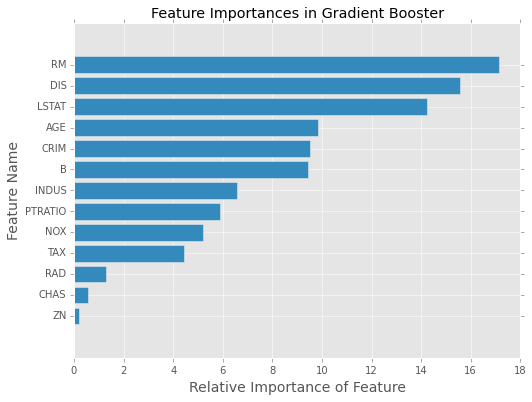
\includegraphics[scale=0.45]{feature-importances}
  \end{figure}
  
\end{frame}
%
\begin{frame}
\textbf{Comments:}\\~\\

\begin{itemize}

\only<1>{
    \item The name "feature importances" is pretty awful.  It invites misinterpretation.  
    \begin{center}
    \textit{Don't reason about things from their names, make sure the statistic actually answers your question}.
    \end{center}
}

\only<2>{
    \item If your model contains both numeric and binary predictors, the importance metric is biased to assign higher values to the numeric predictors (do you see why?).  Try not to compare feature importances across these two classes.
}

\only<3>{
    \item Feature importance rankings can have very high variance.  Make sure any important conclusions are robust to different RNG seeds and training sets.
}

\only<4>{
    \item Make sure your model only includes trees \textit{up to the optimal point}.  Otherwise you'll allocate importance to overfitting.
}

\only<5>{
    \item Dominant features should be treated with suspicion.  They can often be a sign of data leakage.
}
\end{itemize}
\end{frame}
%

\begin{frame}{Partial Dependence Plots}

Visualizations of the effect of a single predictor, averaging out the effects of all the rest

  \begin{figure}
    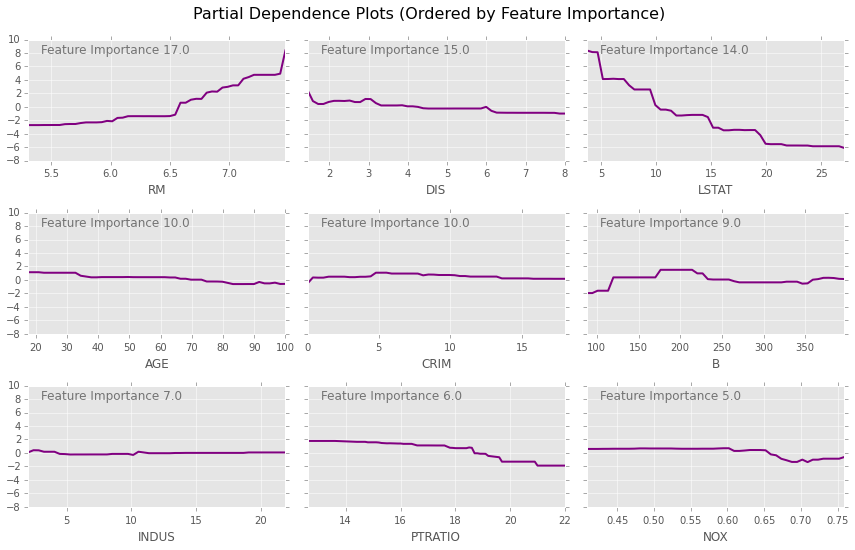
\includegraphics[scale=0.33]{patial-dependence-plots}
  \end{figure}

\end{frame}
%
\begin{frame}
In symbols:

$$ \pd_j(x) = \frac{1}{N} \sum_i f(\overbrace{x_{i1}, x_{i2}}^{\text{The training data points}}, \ldots, \overbrace{x}^{\text{The j'th spot}}, \ldots, x_{iM}) $$
\end{frame}
%
\begin{frame}
By varying the values of two predictors, we can draw partial dependence plots in higher dimensions

  \begin{figure}
    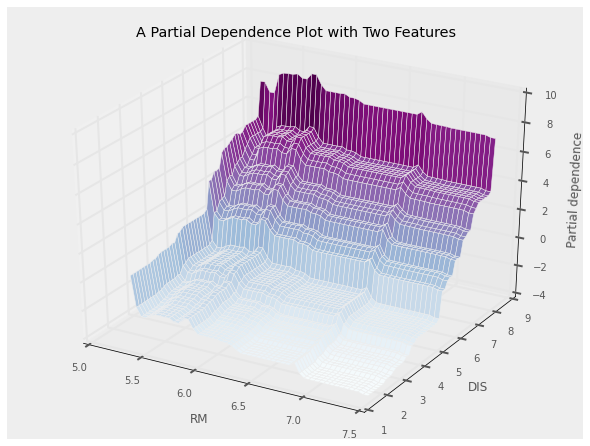
\includegraphics[scale=0.45]{patial-dependence-plot-two-features}
  \end{figure}
 
\end{frame}
%
\begin{frame}
\textbf{Question:} Does it look like any trees split on \textit{both} RM and DIS?

  \begin{figure}
    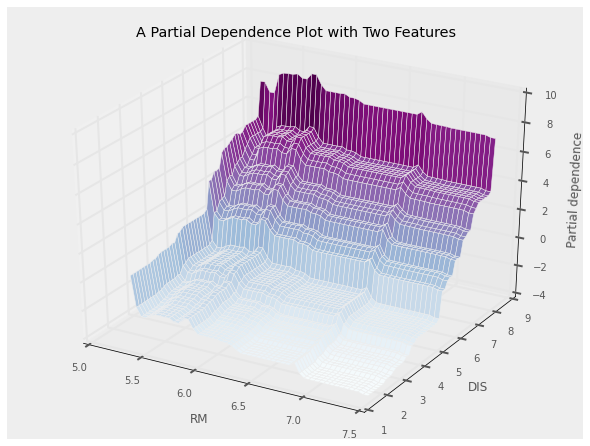
\includegraphics[scale=0.45]{patial-dependence-plot-two-features}
  \end{figure}
 
\end{frame}
%
\begin{frame}
\textbf{Question:} What about AGE and DIS?

  \begin{figure}
    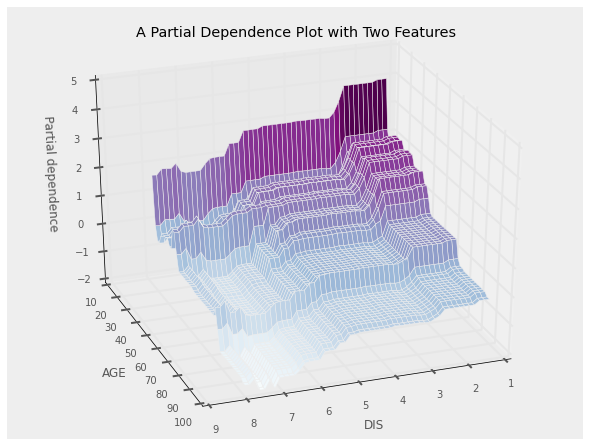
\includegraphics[scale=0.45]{patial-dependence-plot-two-features-with-interaction}
  \end{figure}
 
\end{frame}